\mainsection{\the\numexpr \thechapter + 1 \relax}{Stockage de données}{04/10/2021}

%Théorie :
%Être capable de distinguer un support local d’un support distant.
%Pratique :
%Savoir organiser une arborescence. Comprendre la différence entre un fichier et un dossier. Savoir nommer correctement des fichiers et des dossiers. Distinguer différents types de fichiers. 
%Savoir protéger ses données en mettant en place différents types de sauvegarde. Savoir compresser des données. Utiliser un service de stockage distant. Savoir partager des données. Savoir synchroniser des données par le biais d’outils ou de logiciels appropriés.
%Sensibilisation:
%Sensibiliser à l’évolution et à l’obsolescence des supports et des standards. Savoir que le format de stockage dépend du support et du système d’exploitation.


\vspace{-1cm}
\section{Introduction}
\vspace{-0.5cm}
Les besoins en stockage de données numériques, à l’échelle mondiale, ont été multiplié par plus de vingt au cours de la dernière décennie et devraient dépasser les 50 zettaoctets (1 zettaoctet = $10^{21}$ octets) d’ici fin 2021. A titre de comparaison, toute l'information sous format papier sur terre pourrait être stockée en utilisant environ 0,1 zettaoctet. De même, la capacité mémoire totale des tous les cerveaux humains sur la terre serait d'environ 0,001 zettaoctet (\textit{source: Calcul, mémoire, intelligence ?, Jean-Paul Delahaye}).

Comme le montre l’infographie ci-dessous, cette quantité de données produite aujourd'hui apparaît finalement dérisoire en comparaison avec ce qui est attendu pour les quinze prochaines années. Les prévisions tablent en effet sur une multiplication par trois ou quatre du volume annuel de données créées tous les cinq ans. Avec ce rythme exponentiel de croissance, le seuil astronomique des 2’000 zettaoctets devrait être franchi à l’horizon 2035.
\begin{figure}[h!]
	\centering
	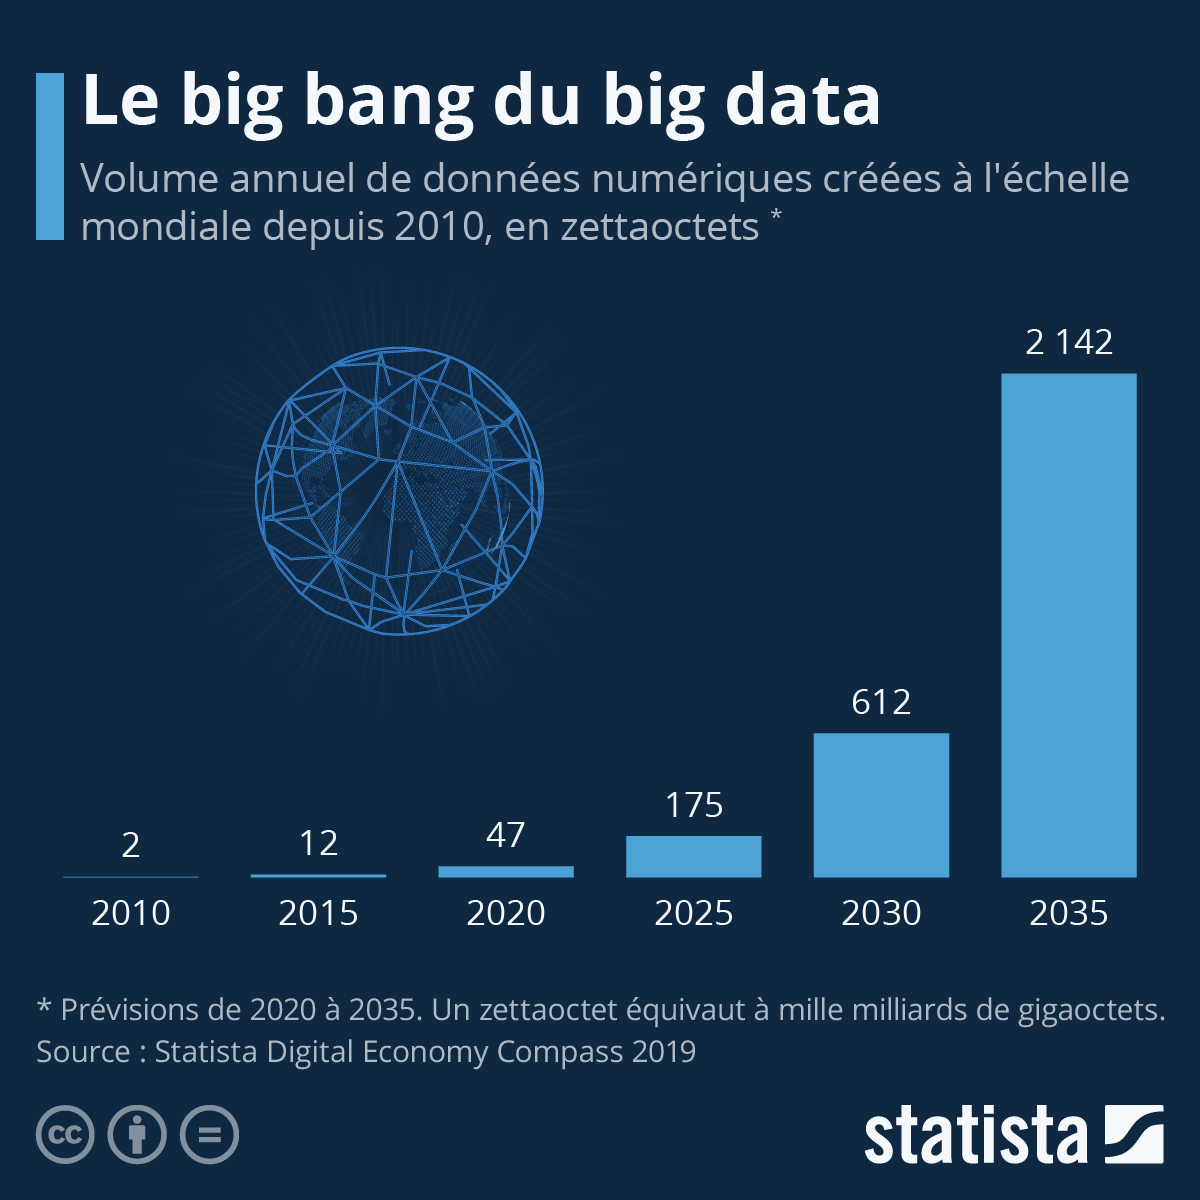
\includegraphics[trim=0 0 0 0,width=0.7\textwidth]{Images/stockage/statista.jpeg}
	\caption{Volume annuel de données numériques créées à l’échelle mondiale depuis 2010, en zettaoctets* (\textit{source: Statista Digital Economy Compass 2019}).}
\end{figure}
Il faudrait se procurer 500 millions de disques durs actuels (100 To) pour être capable de sauvegarder 50 [Zo] ! Cette quantité de données pose autant de problèmes de préservation et d’intégrité des données que de sauvegarde. Sans annoncer les problèmes de places, de consommation électrique, de pollutions dues à la fabrication et au recyclage du matériel vieillissant, de coût et de sauvegarde.


\section{Octet (ou byte) : unités de mesure de la quantité de données}
\begin{myrappel}
	L'{\bf octet} (en anglais {\bf byte}) est une unité d'information composée de 8 bits. Il permet, notamment de stocker un caractère comme une lettre ou un chiffre en utilisant le codage ASCII. Un octet permet de représenter $2^8$, c'est-à-dire 256, valeurs possibles.
\end{myrappel}
Jusqu'en 1998; 1024 octets valaient 1 kilooctet. Et depuis les nouvelles unités standardisées par l'organisme international IEC sont les suivantes :
\begin{center}
	\begin{tabular}{| r || c |  c | c | c | c | c | c |  c |}
		\hline
		Symbole & ko & Mo & Go & To & Po & Eo & Zo & Yo \\ \hline
		Nom & kilooctet & mégaoctet & gigaoctet & téraoctet & pétaoctet & exaoctet & zettaoctet & yottaoctet   \\ \hline
		Valeur & $10^{3}$ & $10^{6}$ & $10^{9}$ & $10^{12}$ & $10^{15}$ & $10^{18}$ & $10^{21}$ & $10^{24}$  \\ \hline
	\end{tabular}
\end{center}

\begin{myremarque}
	Il est encore parfois d'usage d'utiliser les préfixes "kilo", "mega", etc. pour désigner des ordres de grandeur qui sont des multiples de $2^{10}=1024$ en non de $10^3=1000$. Par exemple, un mégaoctet devrait en principe valoir $1000 \cdot 1000$ octets, c'est-à-dire 1'000'000 octets, mais il était d'usage de lui attribuer la valeur de  1024 x 1024 octets, c'est-à-dire 1'048'576 octets... ce qui correspond à une différence de 4.63 \% ! Même si ce mésusage tend à disparaître, cette confusion est encore courante.
\end{myremarque}

\section{Comment estimer la quantité nécessaire d'octets pour stocker de l'information}
La taille d'un fichier va dépendre de 
\begin{itemize}
	\item La quantité d'information\footnote{le mot quantité est à prendre dans son interprétation naïve. Il existe une théorie qui définie de manière rigoureuse le concept de quantité d'information, mais ceci dépasse le cadre du cours}, par exemple:
		\begin{itemize}
			\item Le nombre de caractères pour un fichier texte;
			\item Le nombre de pixels pour une image ou une vidéo;
			\item La longueur d'un enregistrement audio ou vidéo;
			\item etc.
		\end{itemize}
	\item La qualité de l'enregistrement, par exemple:	
		\begin{itemize}
			\item Le nombre de caractères différent que peut contenir notre texte;
			\item Le nombre de couleurs (niveaux de gris) possibles pour une image ou une vidéo;
			\item Le nombre d'images par seconde pour une vidéo;
			\item La fréquence d'échantillonnage ainsi que les niveaux d'encodage du signal pour un enregistrement audio
			\item etc.
		\end{itemize}
	\item Si l'information est compressible, par exemple:
		\begin{itemize}
			\item Si il y a de la redondance dans un texte, peu de caractères sont utilisés ou certains caractères apparaissent très souvent comme le "e" en français;
			\item Si il y a des grandes zones uniformes dans une image;
			\item Si on peut supprimer des fréquences d'un enregistrement audio qui ne sont de toute manière pas détectables par la plupart des oreilles humaines.
			\item etc.
		\end{itemize}	
\end{itemize}
On comprend qu'il est difficile d'estimer la taille d'un fichier en se basant sur l'information qu'il contient. On peut cependant donner un ordre de grandeur de taille de fichier en se basant sur les exemples suivants:
\begin{enumerate}
	\item[-] 3 Ko :        fichier texte (3’000 caractère de texte, environ une page A4)
	
	\item[-] 2 à 3 Mo :   image matricielle 1024x768 \textbf{non compressé} avec les couleurs codées sur 24 bits (un octet pour chacune des couleurs de base : \textit{\textbf{R}ed}, \textit{\textbf{G}reen} et \textit{\textbf{B}lue}).
	\item[-] 30 à 100 Ko :    image matricielle 1024x768 \textbf{compressé} avec le format jpeg.
	\item[-] 50 Mo :     fichier audio qualité CD d’une durée ~3 min (débit 320 kbit/s)
	\item[-] 6 Mo :     fichier audio compressé en  MP3 d’une durée ~3 min (débit 320 kbit/s)
	\item[-] 4 Go :     film ~1h30 (qualité DVD)
	\item[-] 20-25 Go :      film ~1h30 (qualité Blu-ray)
	\item[-] 100 Go et plus :     film résolution 4k
\end{enumerate}


\section{Support de données}
Dans ce chapitre, on s'intéresse seulement à la mémoire persistante. Notre distinction sera basée sur l'usage des supports de mémoire plutôt que sur la technologie utilisée.\\

Quel que soit le type de support, sa taille et son emplacement (local ou distant), ils ont tous certains points communs, comme :
\begin{enumerate}
	\item Les supports contiennent des 1 et des 0 qu’il s’agisse de votre dernier livre ou de votre musique préférée.
	\item Tous les supports ont un schéma d’organisation des données qui est dépendante du système d’exploitation.
	\item Ils ont tous besoin d’être alimentés électriquement pour fonctionner.
	\item Aucun support n’est fiable à 100 \% !
\end{enumerate}

\subsection{Mémoire local}
Les disques dur, ou plus récemment, les disques SSD sont les principaux supports de mémoire persistant des PCs. Ils sont rattachés à l'ordinateur et difficilement transportable. En général, dès que le disque est endommagé, toutes les données sont perdues. Il est toutefois possible d'utiliser des technologies amenant de la redondance, par exemple en copiant chaque donnée à double sur deux disques séparés. Cette stratégie est inefficace si la cause du dysfonctionnement d'un disque est externe, par exemple, un incendie.

\subsection{Mémoire transportable : les supports amovibles}
Il est parfois nécessaire de transporter des données. Dans ce cas, on utilise des supports de mémoire amovibles.
Avant d’avoir les clés USB ou les cartes mémoires que l’on retrouve dans les téléphones, il existait d’autres supports externes. Parmi les premiers supports de données informatiques grand public se trouvait la disquette.

\begin{figure}[ht!]
	\centering
	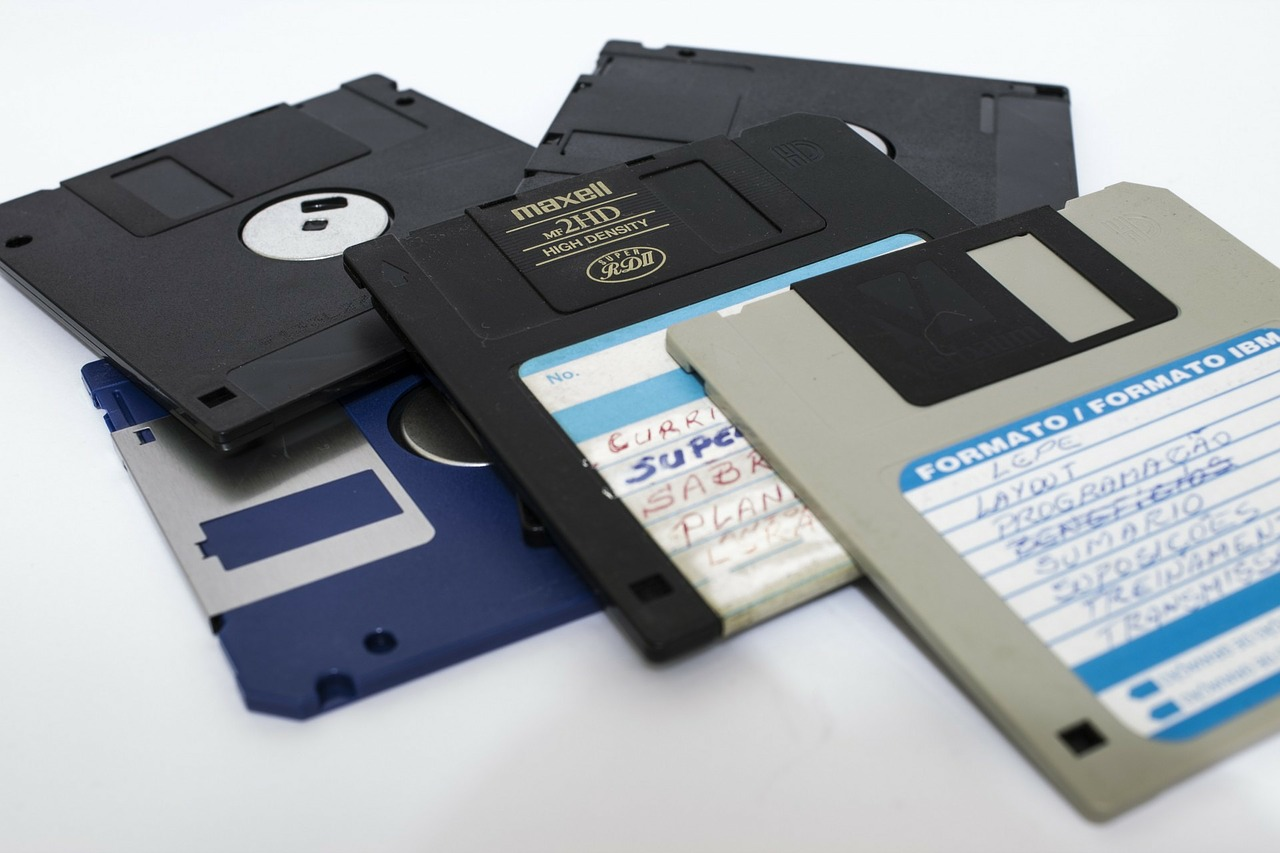
\includegraphics[width=8cm]{Images/stockage/floppy-disk.jpg}
\end{figure}

Inventée dans les années 1970, elle remplaçait les cartes perforées. Quelques exemples de supports amovibles :
\begin{enumerate}
	\item[] 1970 : disquette 8’’ : 1,2 Mo
	\item[] 1970 : disquette 5,25’’ 360k
	\item[] 1980 : disquette 3,5’’: 1,44 Mo, le standard pendant 20 ans !
	\item[] 1990 : CD-ROM 700Mo (d’autre déclinaison jusqu’à 800Mo)
	\item[] 1990 : ZIP : 700Mo
	\item[] 2004 : DVD-ROM : 4,7 Go
	\item[] 2004 : DVD-ROM double couche : 9,4 Go
	\item[] 2006 : Blu-ray 25Go
	\item[] 2006 : Blu-ray double couche 50Go
	\item[] 2000 : clé USB et carte mémoire
\end{enumerate}

\subsection{Supports distants, \textit{solution cloud}}
Avec la multiplication des appareils numérique (PCs, tablettes smartphones, etc.), il est devenu contraignant d'avoirs ses données au même endroit. Par exemple, vous souhaitez accéder à certaines de vos données sur votre tablette à la maison, avec votre téléphone dans le bus ou avec un PC à l'école. 

La rapidité et l'accès à internet à partir de la plupart des ordinateurs ont permis le développement de solutions de stockage accessible à distance. La connexion entre l'ordinateur et un espace de stockage distant, se fait via le réseau internet. On parle de support de mémoire distant ou en nuage (\textit{cloud} en anglais).

\begin{myremarques}
	\item Le terme « cloud » est une forme abrégée de « cloud computing » ou l’informatique en nuage. Un cloud est constitué de serveurs situés à distance et accessibles de n’importe où et à n’importe quel moment via une connexion Internet sécurisée et protégée.
	\item Le terme dématérialisation de l'information est souvent évoquée, mais il ne faut pas s'y tromper, il existe quand même quelque part un support matériel (ou plusieurs) qui stocke vos données. 
\end{myremarques}

\begin{figure}[ht!]
	\centering
	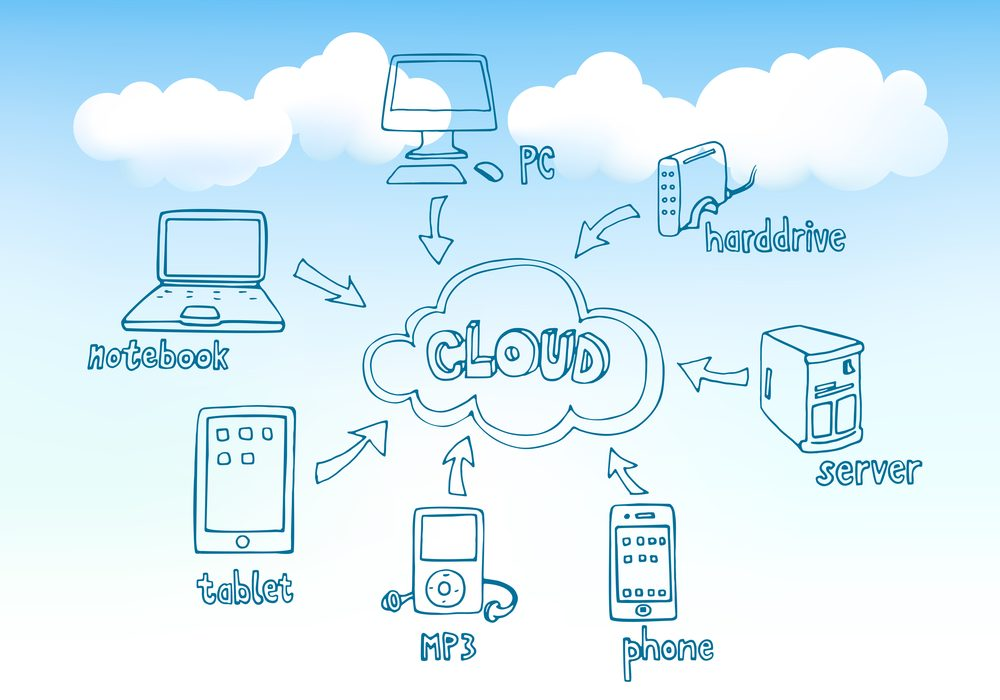
\includegraphics[width=10cm]{Images/stockage/cloud_storage.jpg}
	
\end{figure}

\subsubsection{Avantages et inconvénients d'une solution cloud pour stocker vos données}
\textbf{Exemple d'une offre}\\ L’entreprise \textit{Cloud Prenium} propose un abonnement de 5 chf par mois pour 1 To de place pour vos données. 

\textbf{Question : }Quels sont les avantages et les inconvénients d'une solution en nuage comme celle proposée par \textit{Cloud Prenium}?

\textbf{Avantages principaux du cloud :}
\begin{enumerate}
	\item[+] Vos données sont accessibles partout, à condition d’être connecté à Internet. Vos données sont donc accessibles depuis votre smartphone, votre PC, etc.
	\item[+] Possibilité de partager ses données. De plus, certains logiciels permettent la modification simultanée et gèrent l’accès concurrent.
	\item[+] Aucun investissement ni installation préalable requise, juste le prix de l’abonnement. Il vous suffit en général d’un navigateur web pour accéder à vos données.
	\item[+] Maintenance, sécurisation des données et mises à jour effectuées par le fournisseur.
	\item[+] Souplesse dans l’espace loué. Si vous avez besoin de 2 To, vous pourrez faire évoluer votre abonnement.
	\item[+] En cas de panne de votre ordinateur personnel, vous ne perdez pas les données qui sont dans le cloud.
\end{enumerate}
\textbf{Inconvénients principaux du cloud :}
\begin{enumerate}
	\item[-] Pas de contrôle total d’accès aux données par rapport à l’entreprise \textit{Cloud Prenium}. Confidentialité des données compromise si aucun outil n’est mis en place pour protéger les documents sensibles ;
	\item[-] Savez-vous où sont réellement hébergées vos données ?
	\item[-] Dépendance avec l’entreprise. Si \textit{Cloud Prenium} fait faillite ou son centre de données brule\footnote{\url{https://www.zdnet.fr/actualites/incendie-du-datacenter-de-strasbourg-polemique-autour-des-possibles-negligences-d-ovhcloud-39920937.htm}} que se passe-t-il ? 
	\item[-] Risque de cyberattaques si les données ne sont pas bien protégées.
	\item[-] Obligation d’être connecté à Internet. Le service peut être dégradé si la liaison n’est pas fiable.
	\item[-] Accès aux fichiers plus lents que sur un support local.
	\item[-] Impact écologique : par ses serveurs nécessaires au fonctionnement du cloud, ce dernier induit une consommation d’énergie croissante.
\end{enumerate}
\begin{eclairage}
	En 2016, il était estimé qu'environ 10\% de la production d'électricité du monde était destinée au secteur du numérique. Les \textit{centres de données} accaparaient environ 20\% de ces ressources (source : association negaWatt). 
\end{eclairage}

\section{Stratégie de sauvegarde}
\subsection{Introduction}
Aucun support de stockage n’a une durée de vie illimitée et aucun support de stockage n’est fiable à 100\%. Le risque zéro n’existe pas. Une perte de données numériques est donc très vite arrivée. Les causes principales sont:
\begin{itemize}
	\item des défaillances techniques matérielles comme un disque dur en panne ou une clé usb qui n’est plus accessible;
	\item des défaillances logicielles comme un fichier corrompu suite à une écriture erronée par le système d’exploitation, une erreur de synchronisation;
	\item des défaillances humaines comme un fichier effacé, un fichier écrasé ou une clé usb perdue;
	\item des catastrophes naturelles comme des incendies ou des dégâts des eaux;
	\item des programmes malveillants et des attaques de virus ou de ransomware;
	\item le vol du matériel comme votre téléphone portable, un disque d’un serveur, une clé usb, une carte mémoire;
\end{itemize}
Le monde professionnel indique une durée de vie moyenne de 5 ans pour un disque dur mécanique ou un disque type SSD. Une clé usb ou une carte mémoire de qualité pourrait tenir 10 ans. Le cloud offert par les entreprises de stockage a une durée de vie virtuellement illimitée (voir les inconvénients principaux du cloud).

\subsection{Stratégie 3-2-1 de sauvegarde de données}

La stratégie de sauvegarde 3-2-1 représente le b-a-ba et le minimum de la protection des données. Mise au point par un photographe souhaitant protéger ses clichés dans les années 1920, cette stratégie est devenue une référence, car elle permet une protection optimale des données, quel que soit leur format.

Le concept de base de la stratégie 3-2-1 repose sur trois principes :
\begin{enumerate}
	\item[->] \textbf{{\huge 3} copies de vos données:} La stratégie recommande d’avoir 2 copies plus la source. Avec trois copies dont deux sauvegardes, le risque que les trois copies aient un problème en même temps est très faible surtout si elles sont stockées sur des supports différents.
	
	\item[->] \textbf{{\huge 2} supports différents:} La notion de supports différents est essentielle quand on parle de données numériques, car quel est l’intérêt d’avoir deux sauvegardes si elles sont stockées sur le même support ? En cas d’incident, toutes les données seraient perdues. Il est donc important que la source et au moins une de ses copies soient sauvegardées sur des supports différents.
	
	\item[->] \textbf{{\huge 1} copie hors site:} Quel que soit le support (NAS, disque dur externe, lecteur de bande, etc.), aucune stratégie de sauvegarde de données numériques ne peut être considérée comme sûre si au moins une des copies n’est pas stockée « hors site ». Le récent incendie du 10 mars 2021 d’OVH en est la preuve. En effet, certains utilisateurs avaient leur site en production sur un serveur et leurs copies sur un autre serveur. Certes, les copies étaient sur des supports différents, mais elles étaient stockées dans le même datacenter. Comme une grande partie du site contenant ces serveurs a cessé de fonctionner à cause de l’incendie, aucune des copies n’était utilisable. Or, si au moins une de ces copies avait été stockée chez un autre hébergeur (hors site), ces utilisateurs auraient pu rétablir rapidement leurs services.
\end{enumerate}

Malgré tout les stratégies de sauvegarde ont leurs limites ! La quantité de données à sauvegarder peut prendre trop de temps et poser des problèmes d’intégrité des données. L’externalisation des sauvegardes selon la méthode 3-2-1 soulève aussi la question de la protection des données. 

Et si vous avez bien conservé votre donnée numérique. Serez-vous capable de la relire ?
